\documentclass[12pt]{article}
\usepackage{times}
\usepackage{geometry}
\usepackage{listings}
\usepackage{color}
\usepackage{xcolor}
\usepackage[most]{tcolorbox}
\definecolor{bg}{RGB}{240,248,255}
 
\definecolor{codegreen}{rgb}{0,0.6,0}
\definecolor{codegray}{rgb}{0.5,0.5,0.5}
\definecolor{codepurple}{rgb}{0.58,0,0.82}
\definecolor{backcolour}{rgb}{0.95,0.95,0.92}
 

\lstdefinestyle{CStyle}{   
    commentstyle=\color{blue},
    keywordstyle=\color{magenta},
    numberstyle=\tiny\color{gray},
    stringstyle=\color{purple},
    basicstyle=\footnotesize,
    breakatwhitespace=false,         
    breaklines=true,                 
    captionpos=b,                    
    keepspaces=true,                 
    numbers=left,                    
    numbersep=5pt,                  
    showspaces=false,                
    showstringspaces=false,
    showtabs=false,                  
    tabsize=2,
    language=C,
    frame=single
}
 
\lstset{style=CStyle}

\geometry{letterpaper, portrait, margin=0.2in}
\usepackage[utf8]{inputenc}
\usepackage{enumitem,amssymb}
\usepackage{ragged2e}
\usepackage{pythonhighlight}
\newlist{thematic}{itemize}{8}
\setlist[thematic]{label=$\square$}\renewcommand{\baselinestretch}{0.6} 
\usepackage{pifont}
\newcommand{\cmark}{\ding{51}}%
\newcommand{\xmark}{\ding{55}}%
\newcommand{\done}{\rlap{$\square$}{\raisebox{2pt}{\large\hspace{1pt}\cmark}}%
\hspace{-2.5pt}}
\newcommand{\wontfix}{\rlap{$\square$}{\large\hspace{1pt}\xmark}}
\usepackage{xparse}
\NewDocumentCommand{\code}{v}{%
\texttt{\textcolor{blue}{#1}}%
}
\renewcommand{\baselinestretch}{0.6} 
\usepackage{graphicx}
\graphicspath{ {./imgs/} }



\begin{document}
\begin{figure}
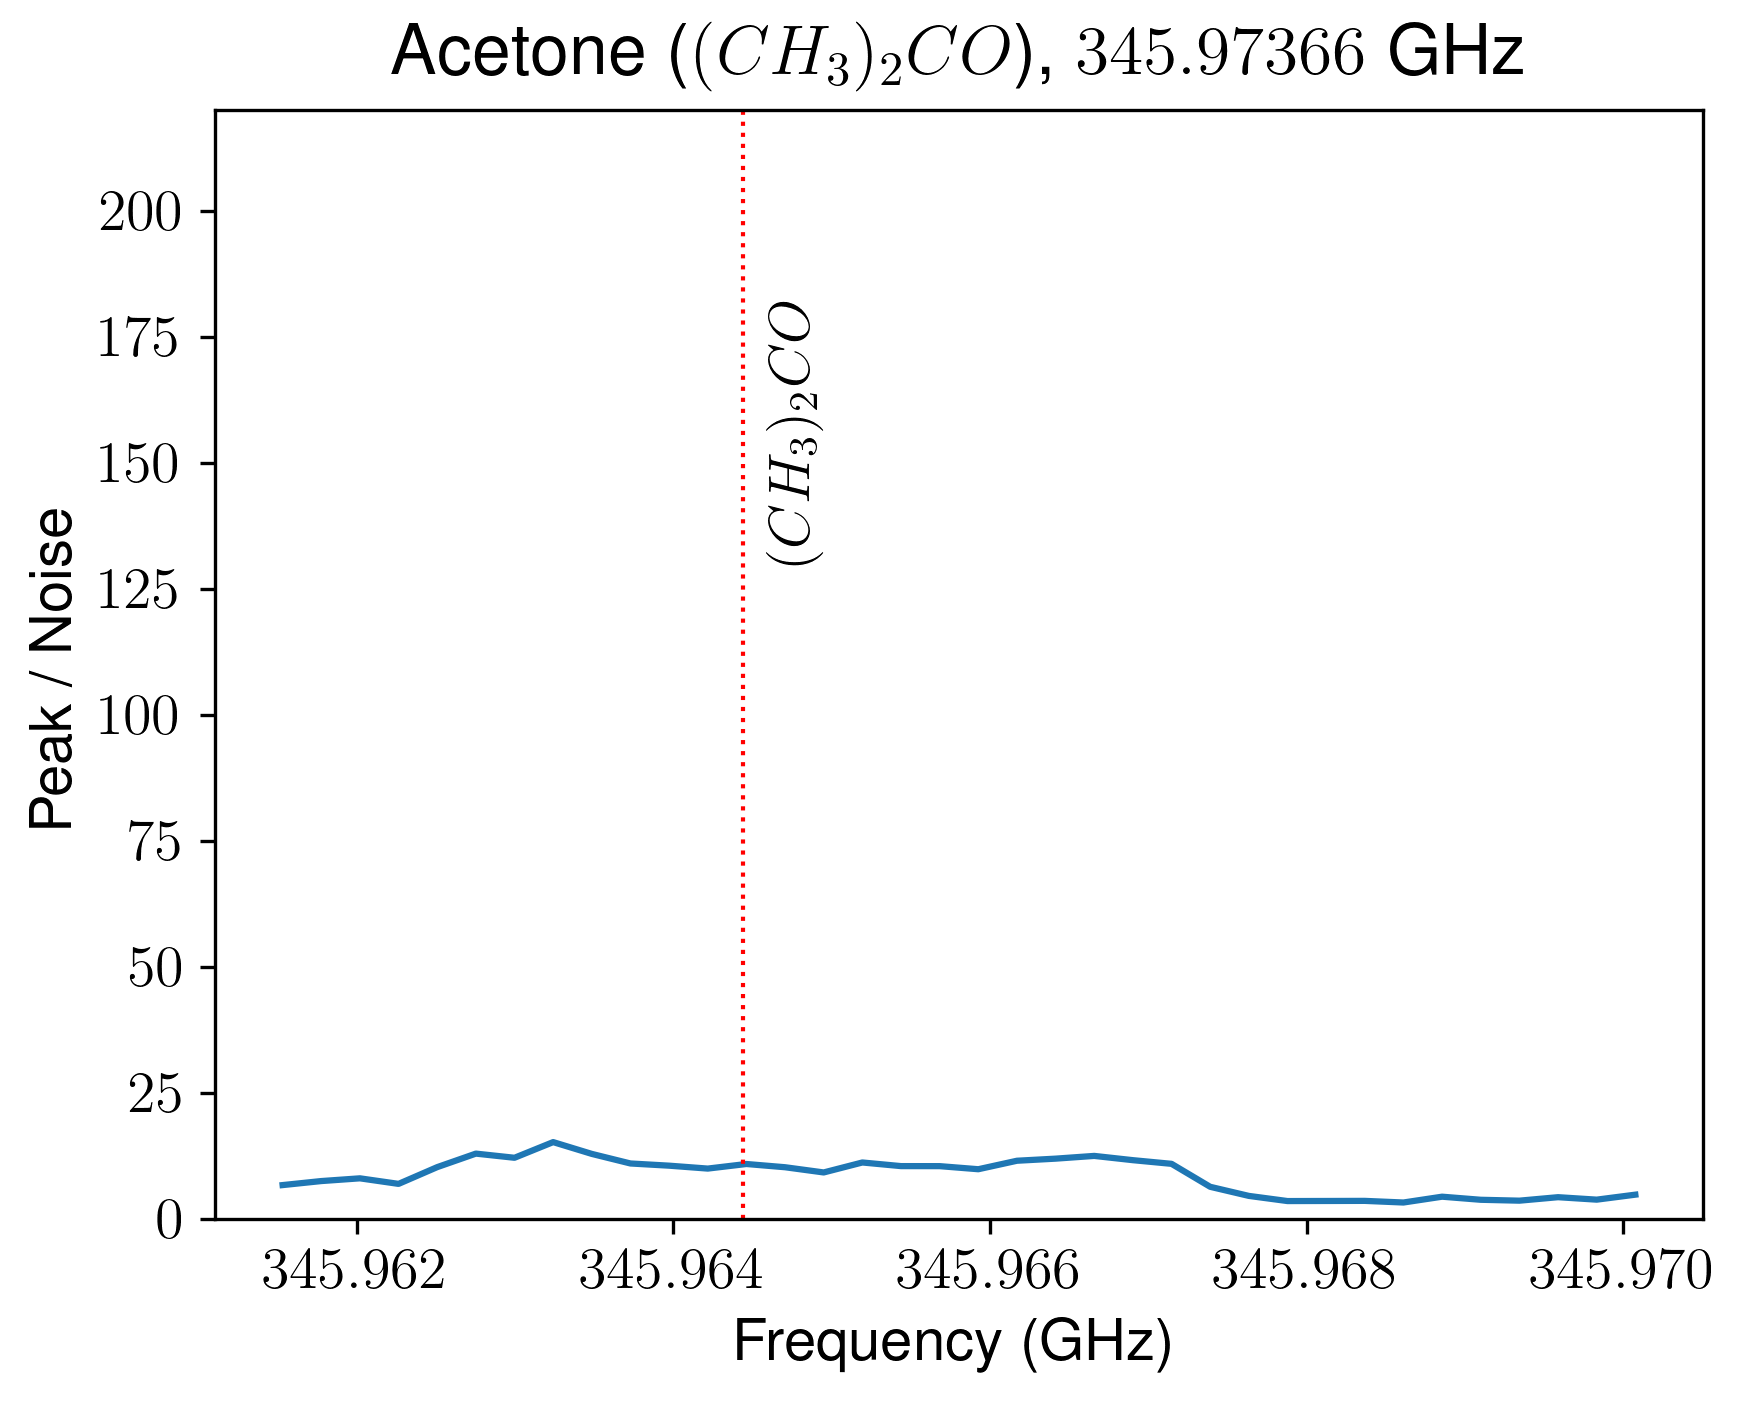
\includegraphics[width=0.245\textwidth]{spw3_(CH3)2CO}
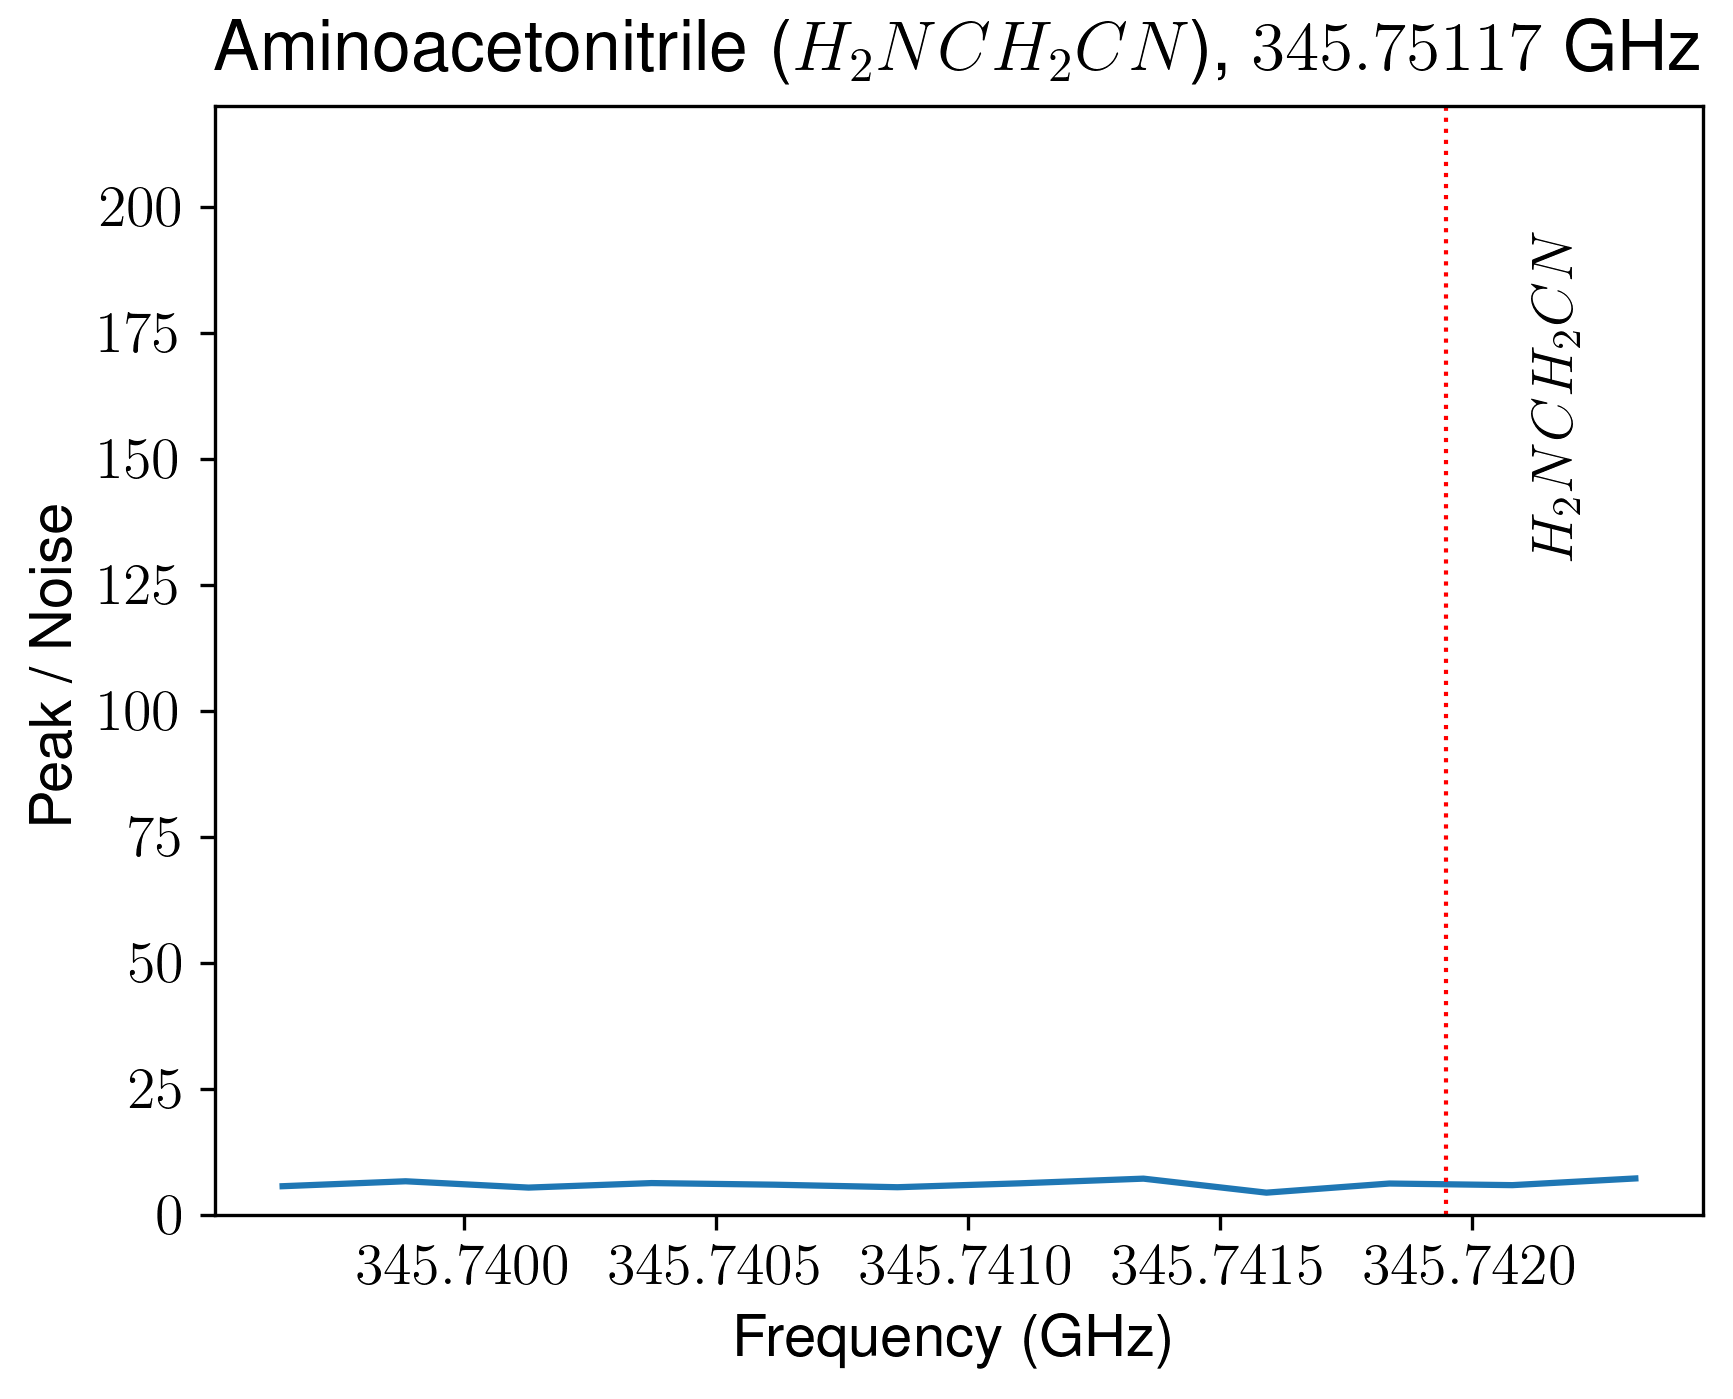
\includegraphics[width=0.245\textwidth]{spw3_H2NCH2CN}
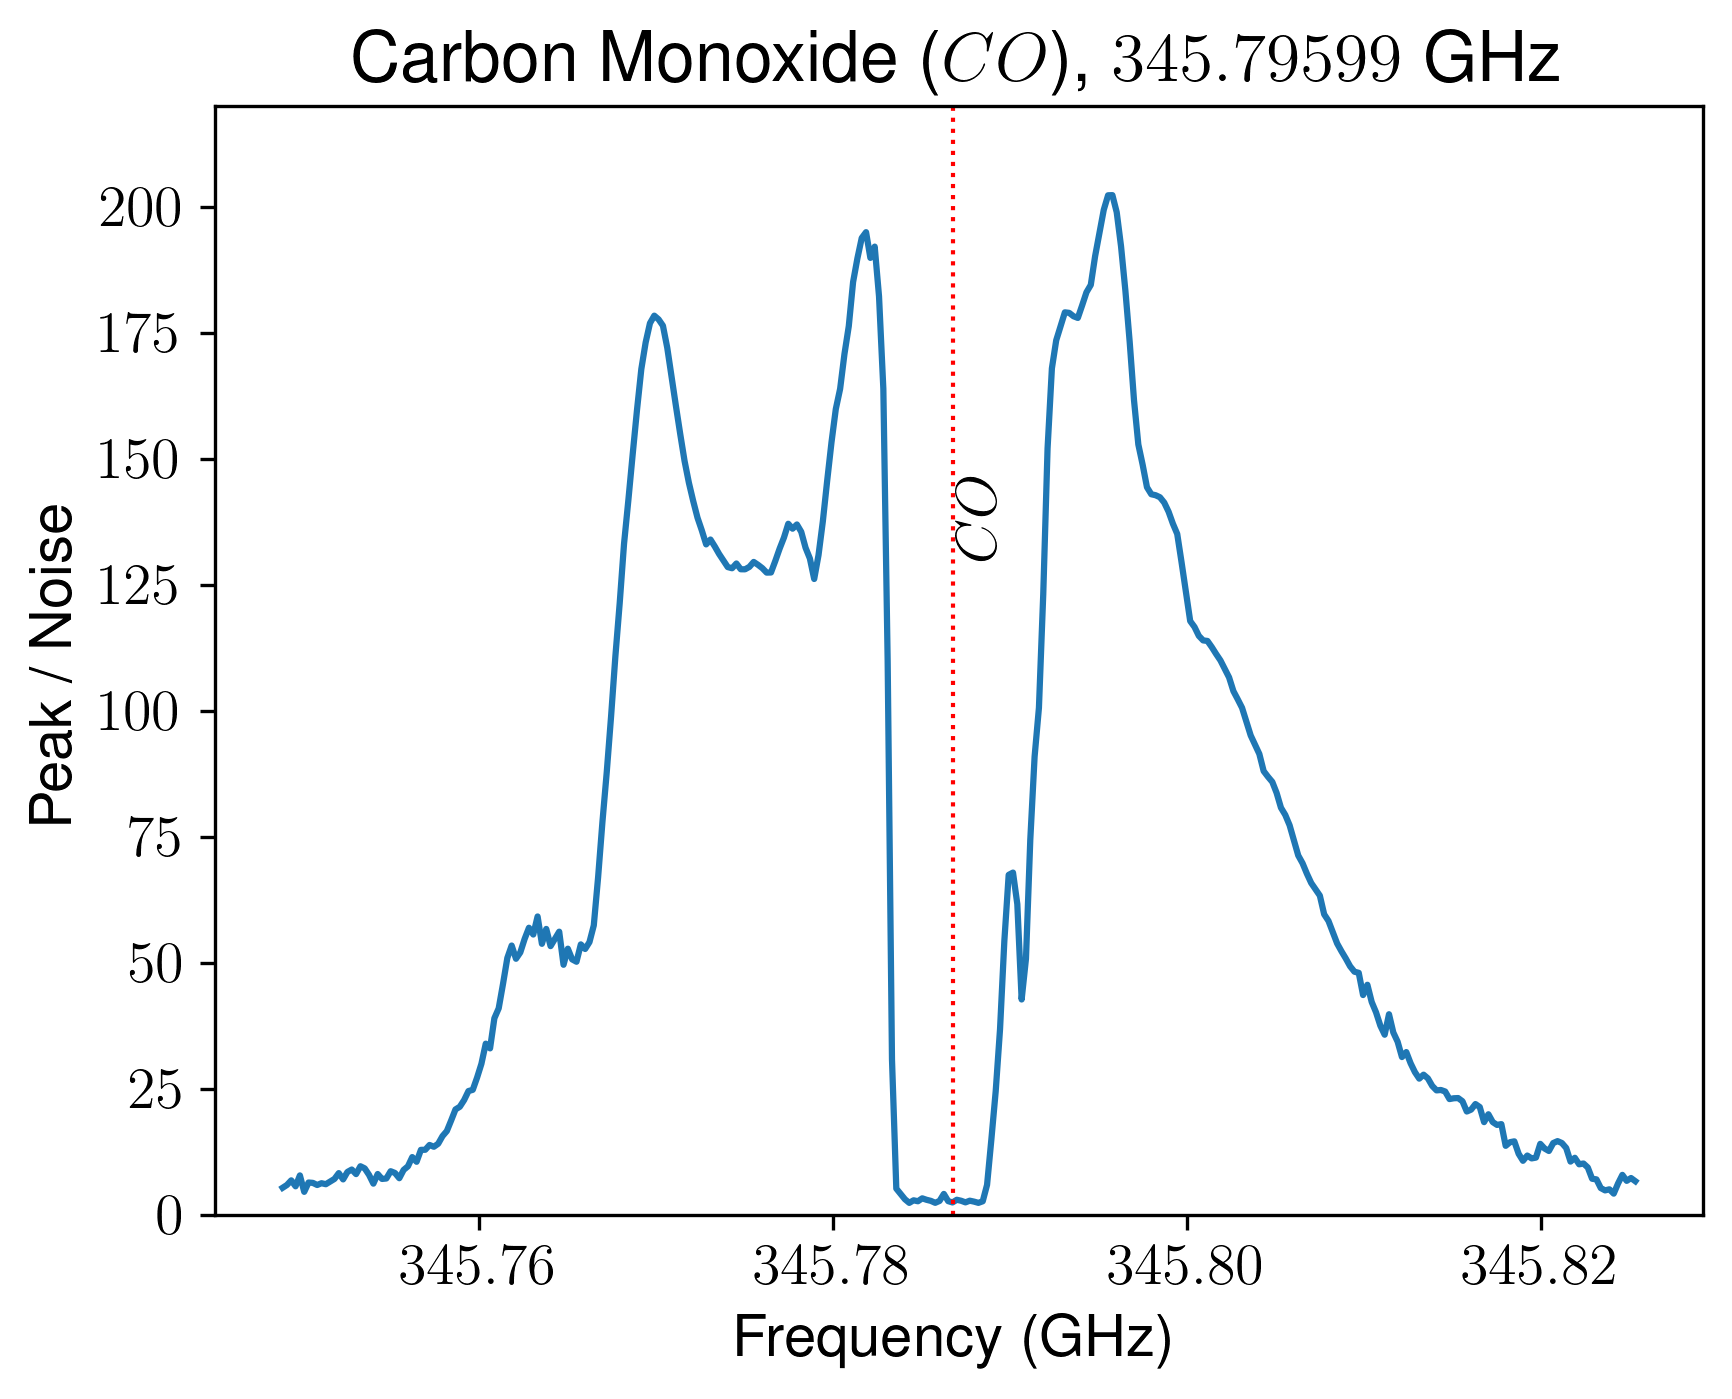
\includegraphics[width=0.245\textwidth]{spw3_CO}
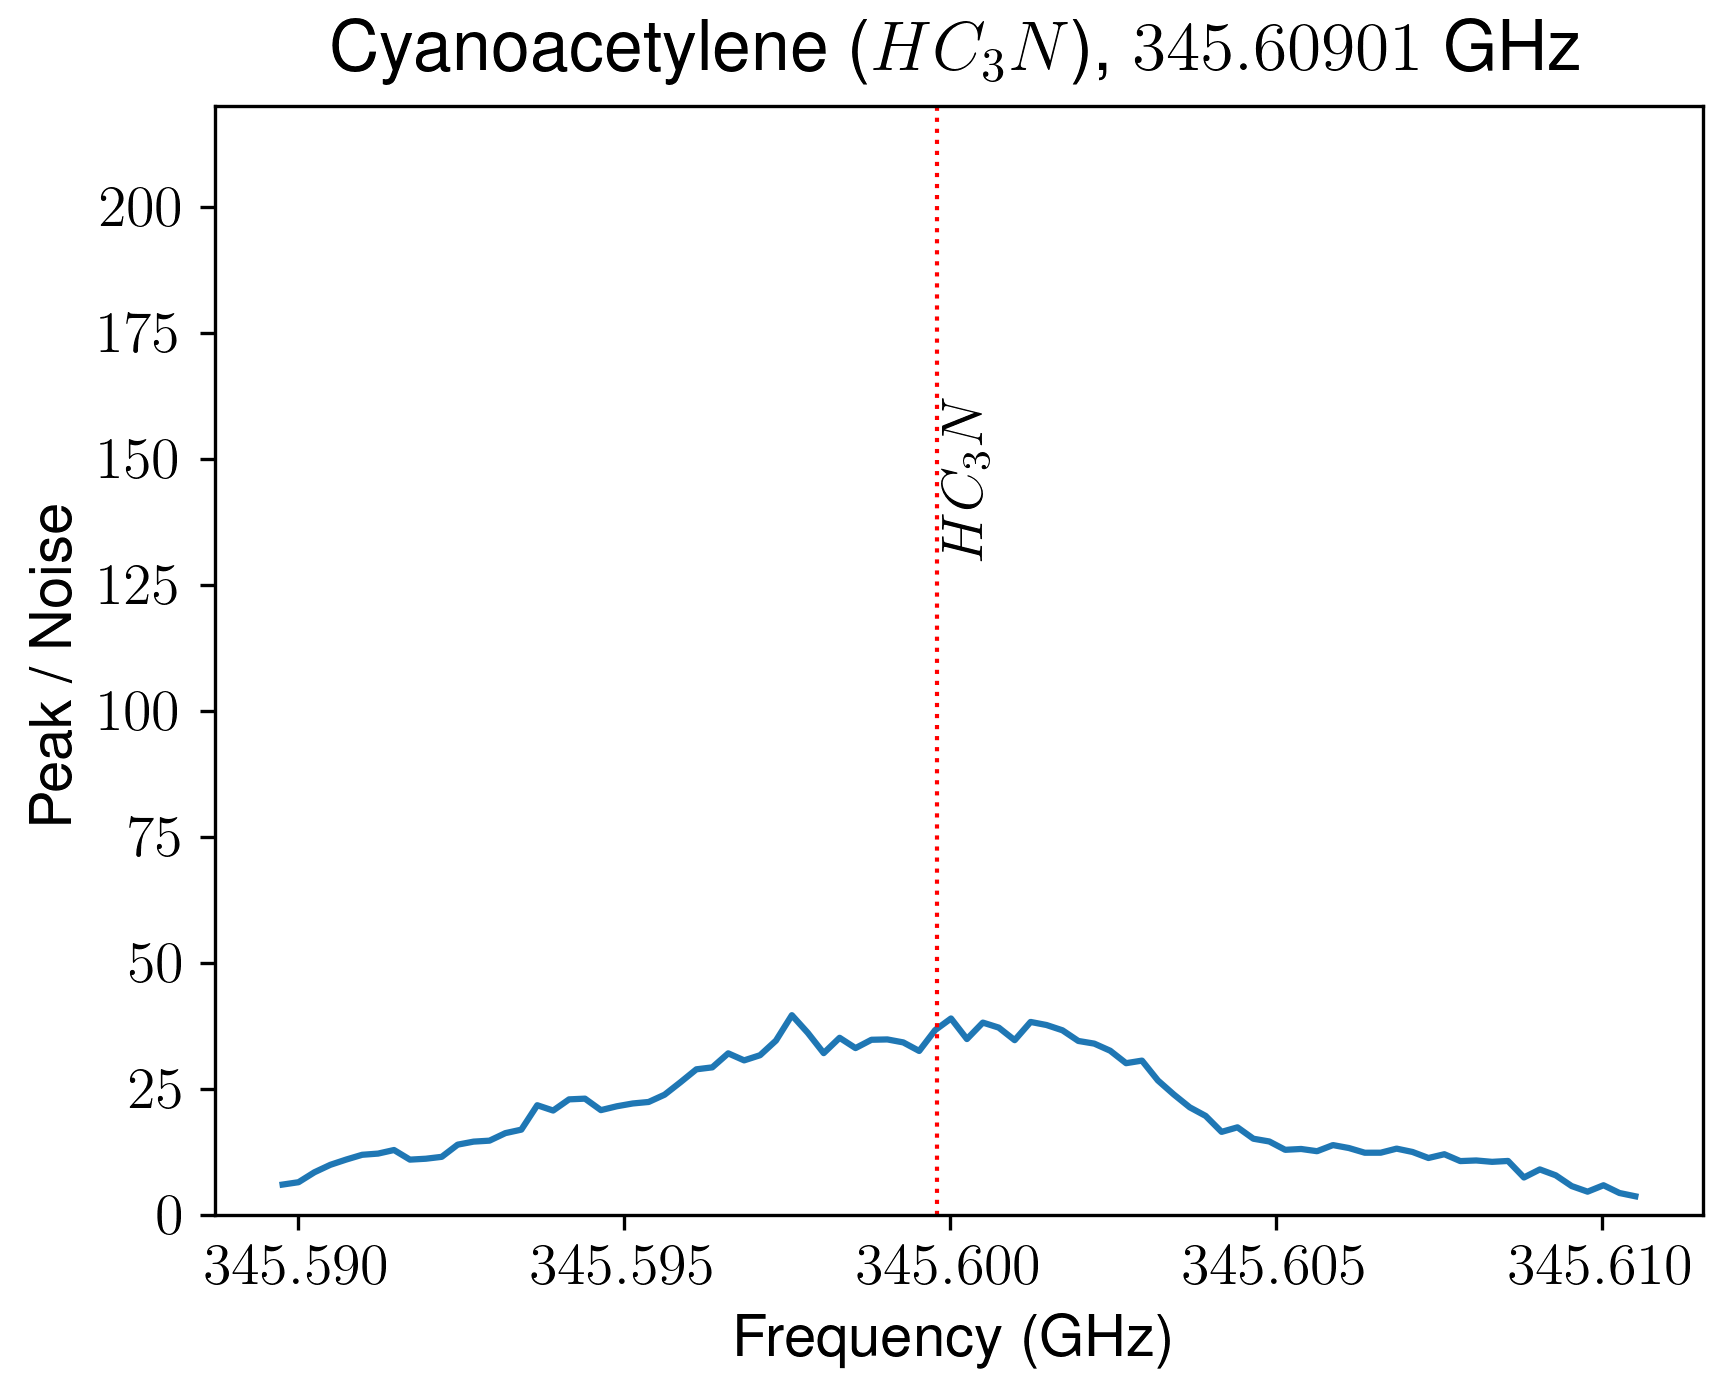
\includegraphics[width=0.245\textwidth]{spw3_HC3N}
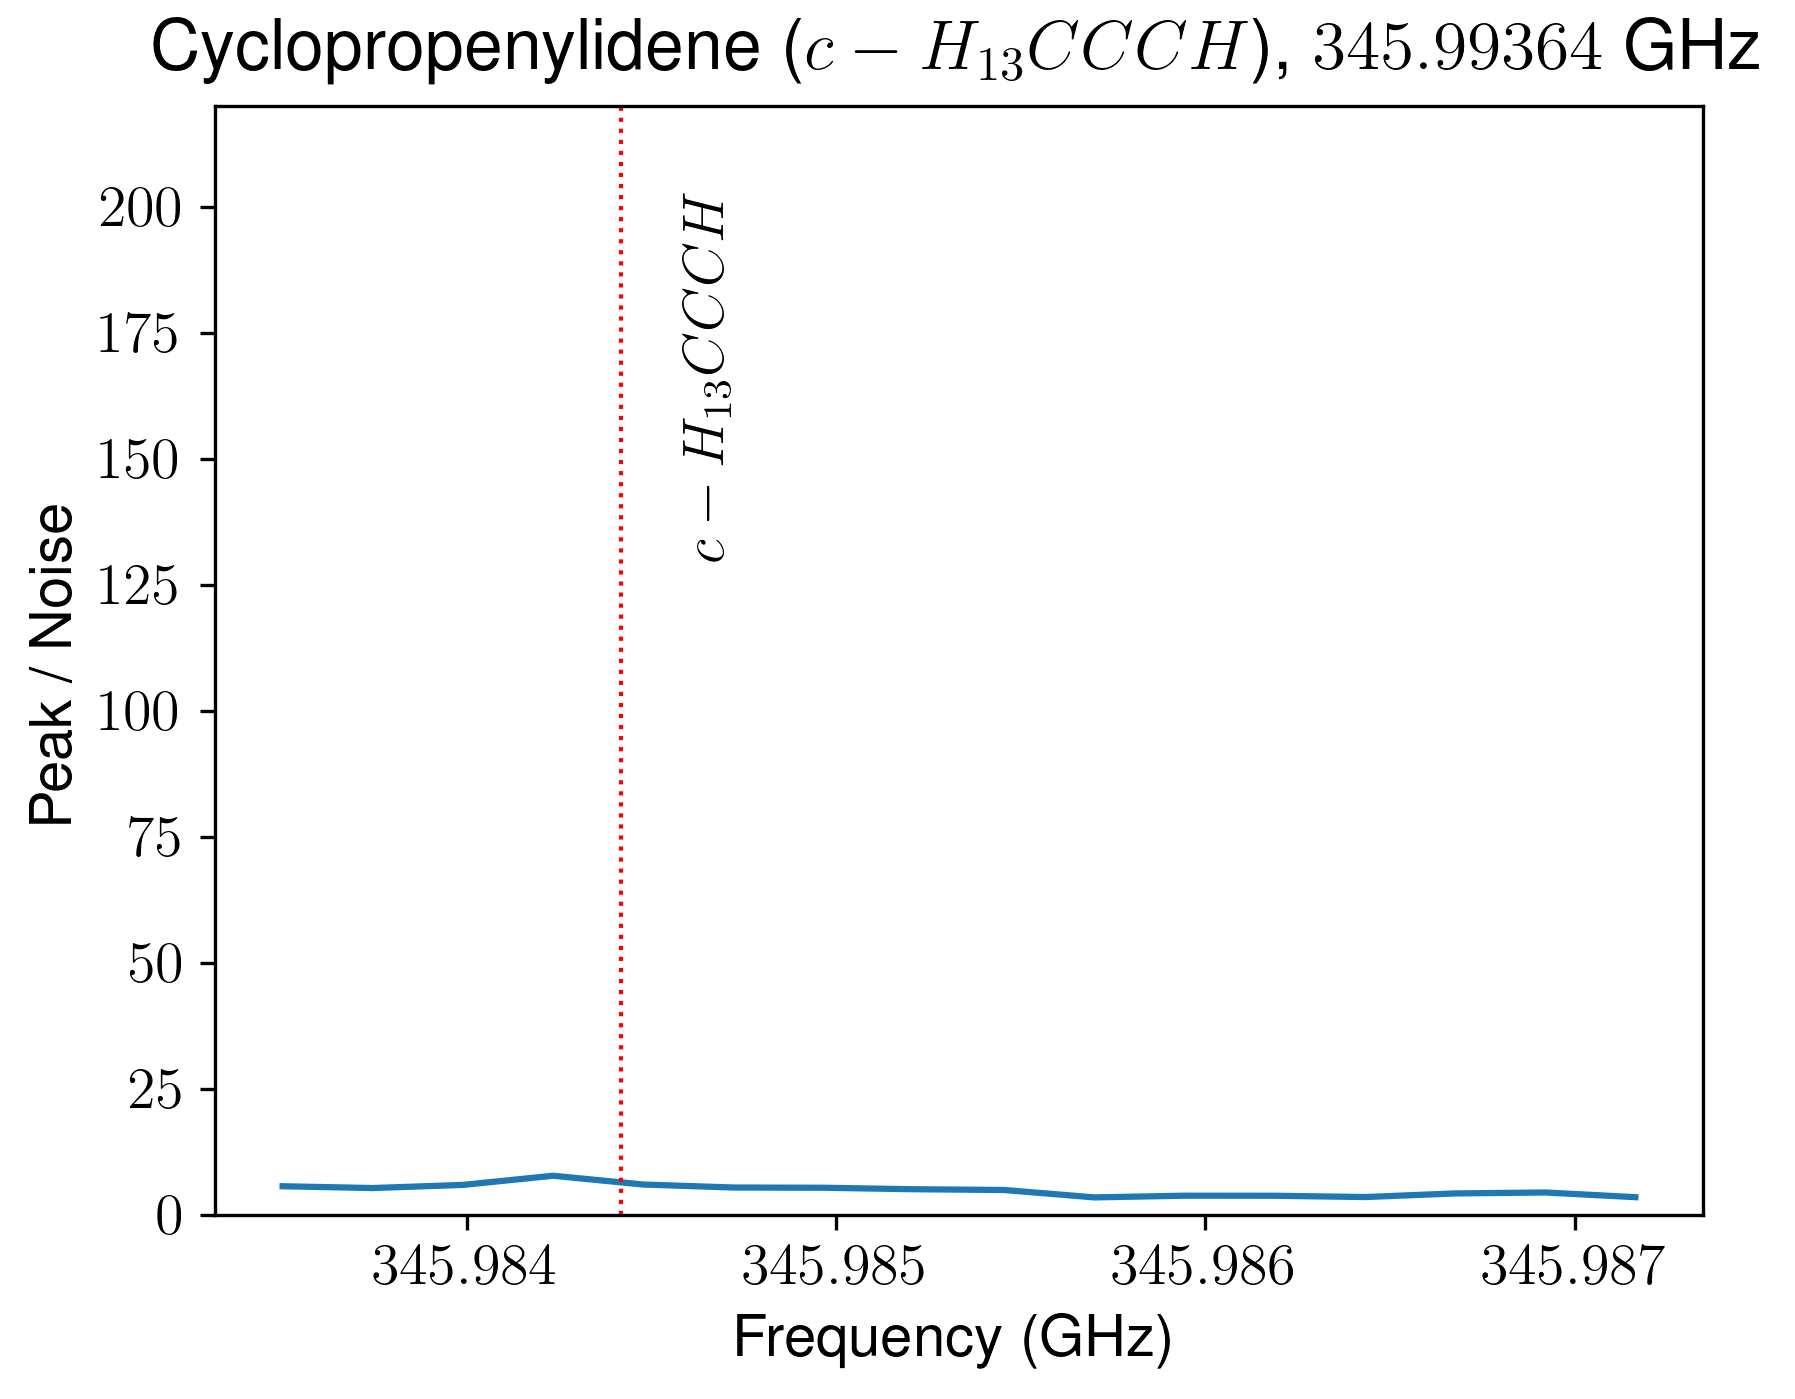
\includegraphics[width=0.245\textwidth]{spw3_c-H13CCCH}
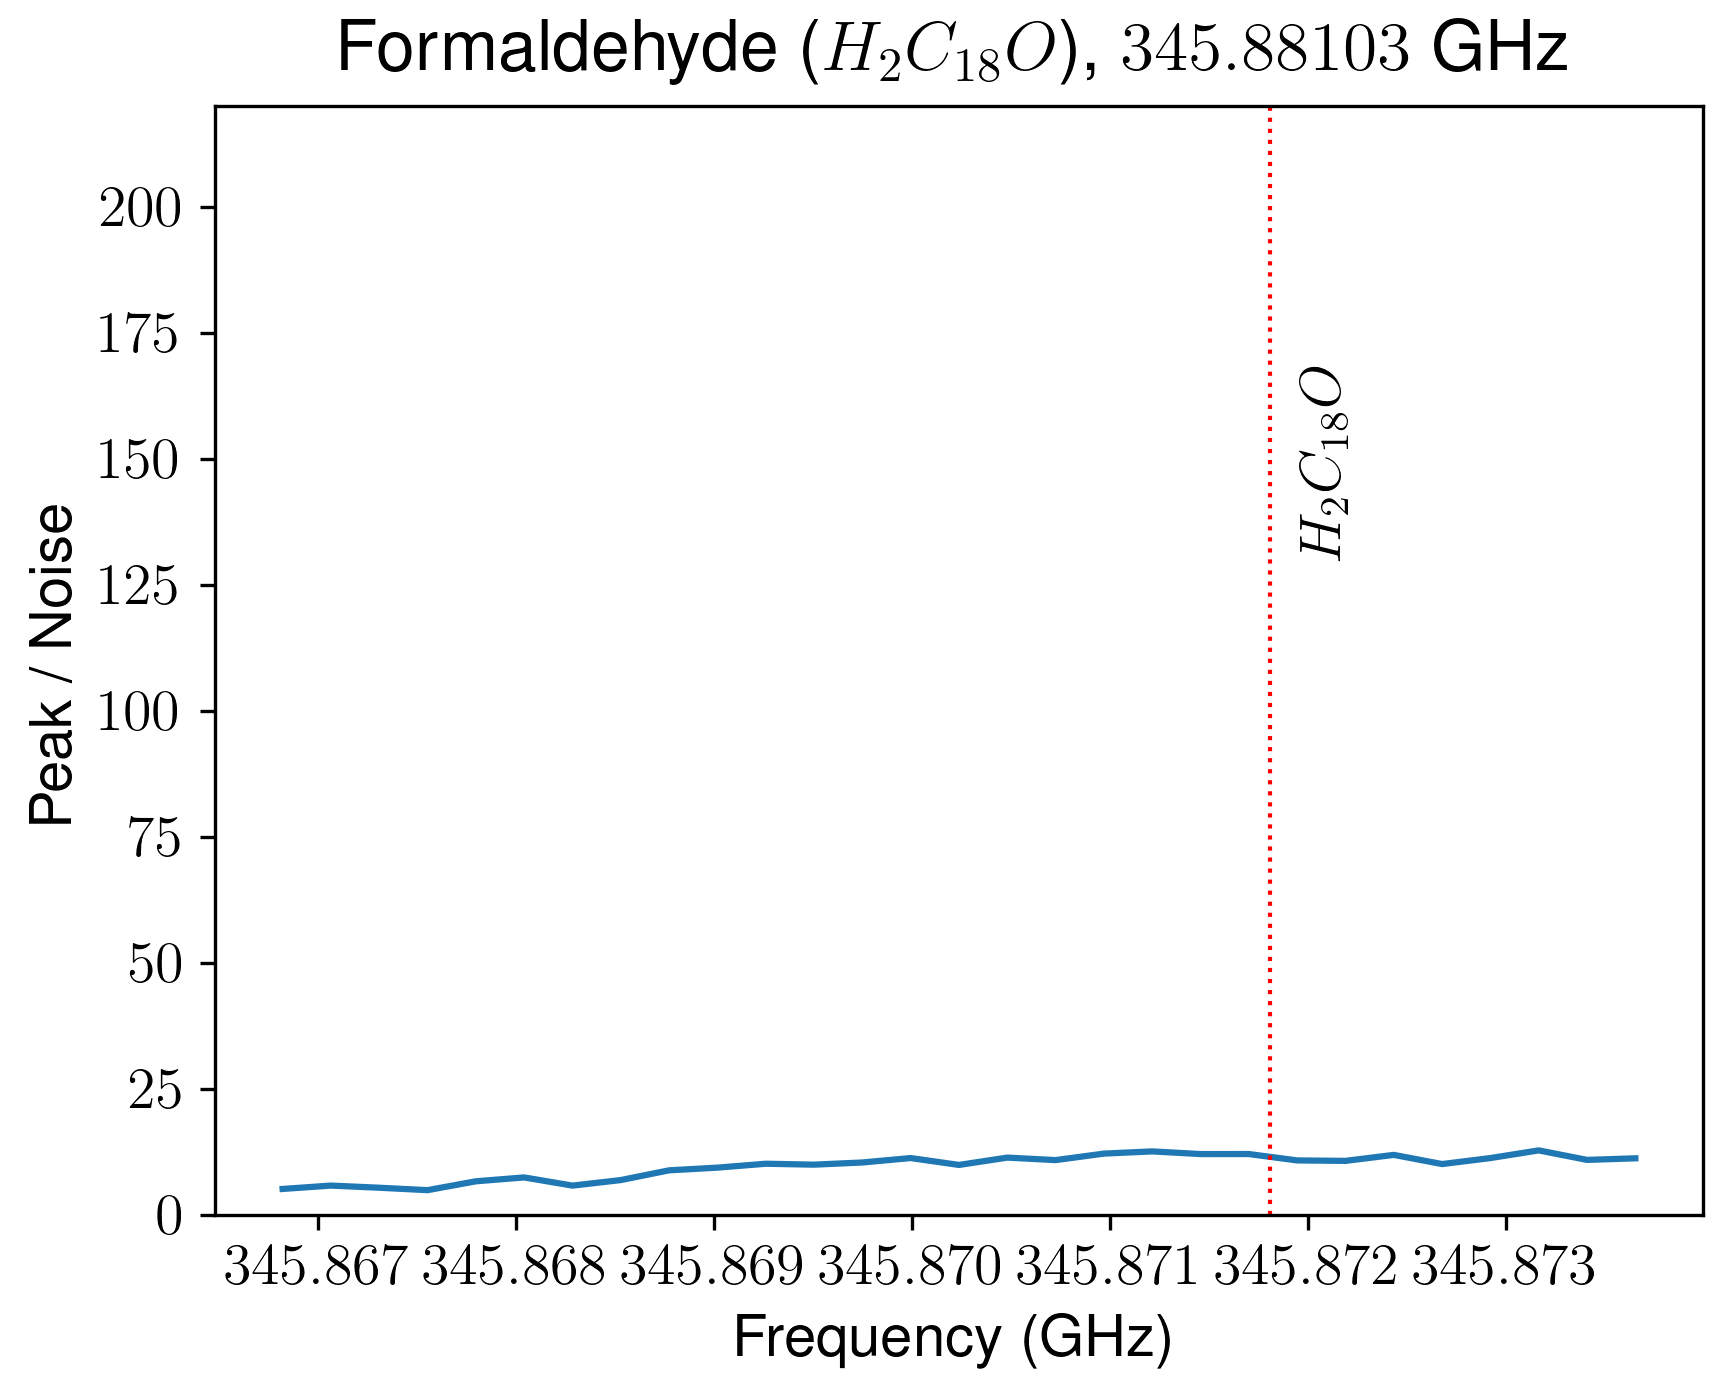
\includegraphics[width=0.245\textwidth]{spw3_H2C18O}
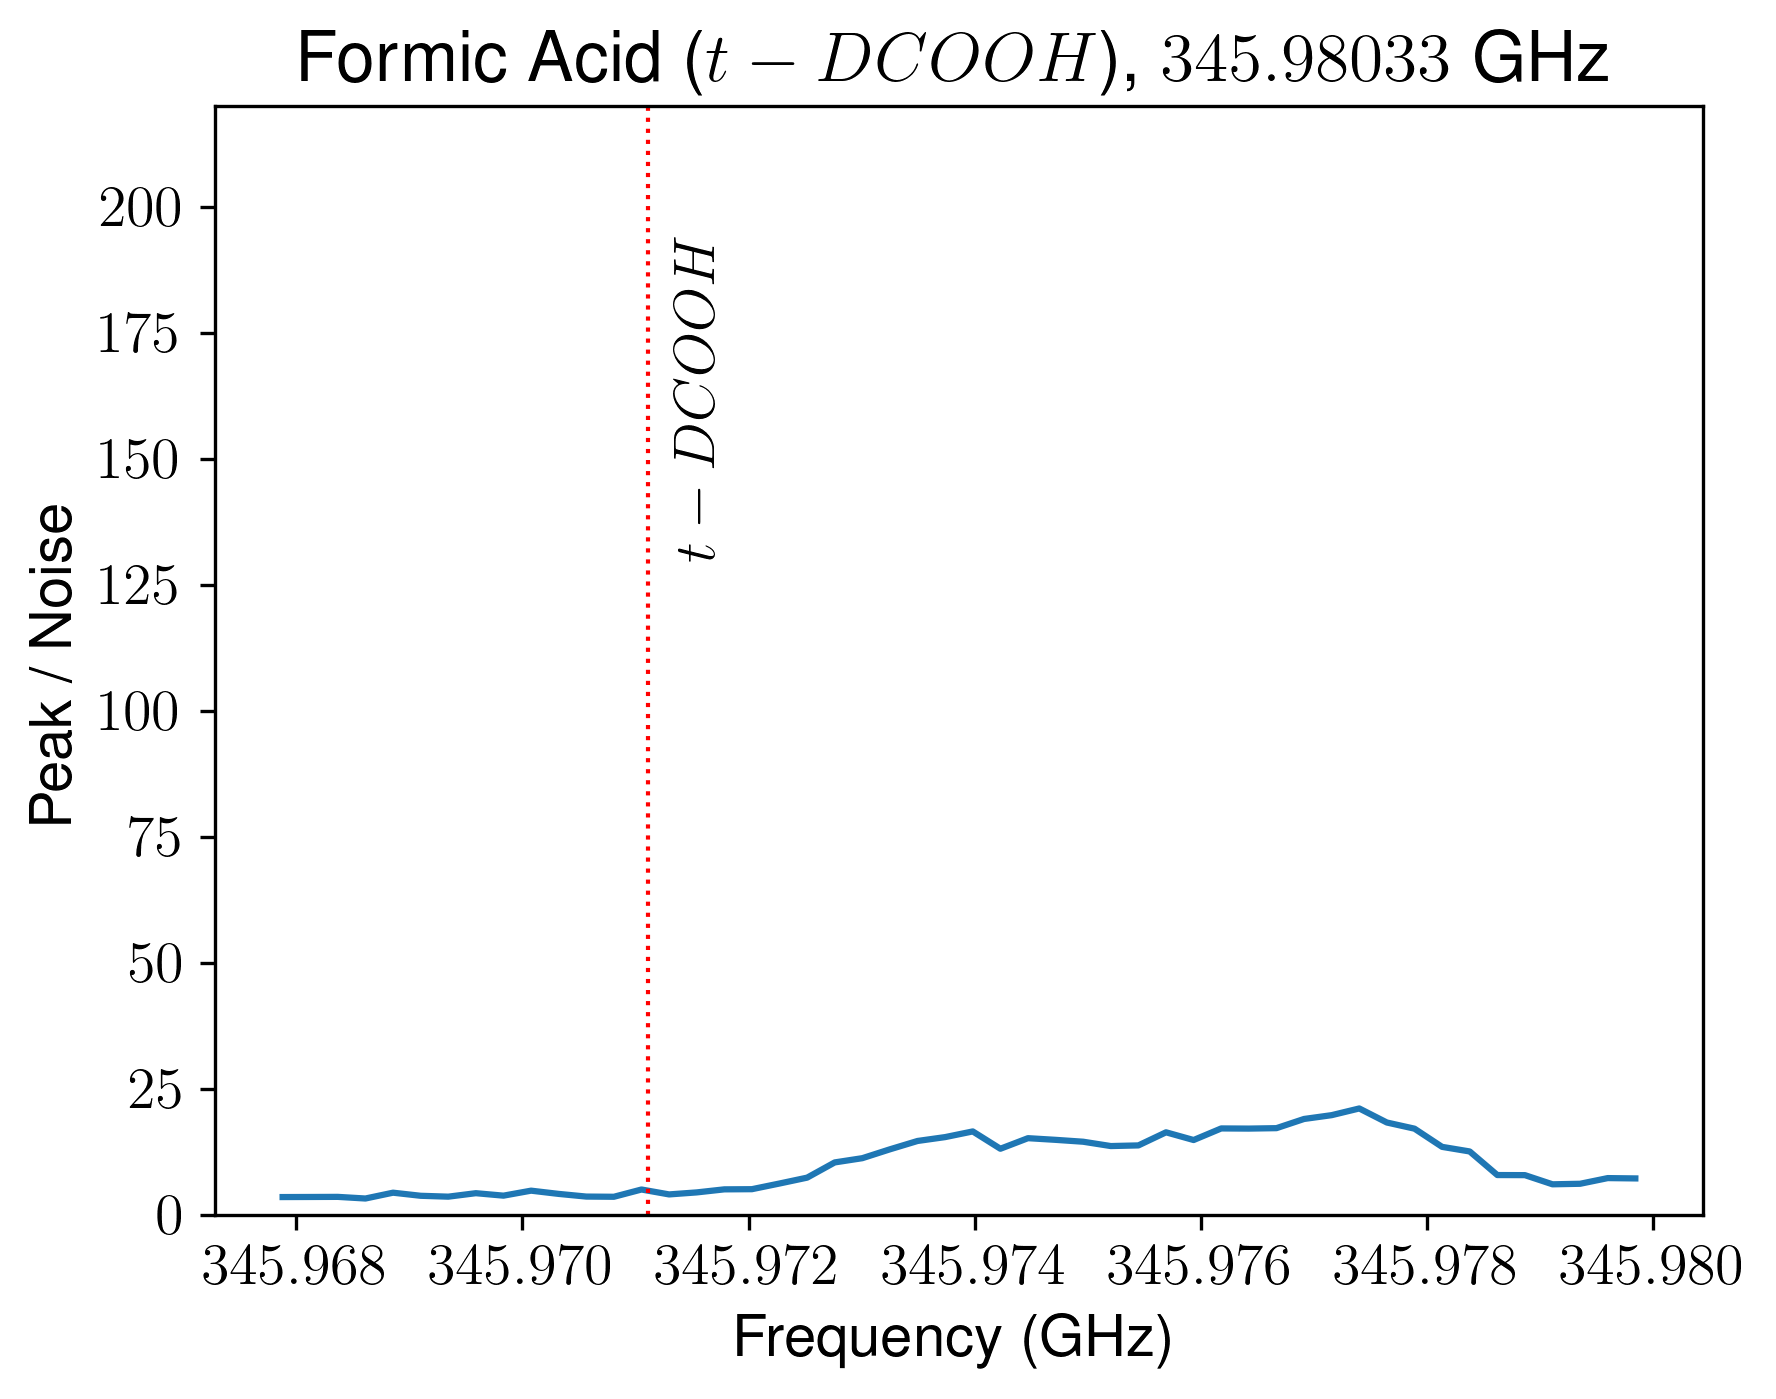
\includegraphics[width=0.245\textwidth]{spw3_t-DCOOH}
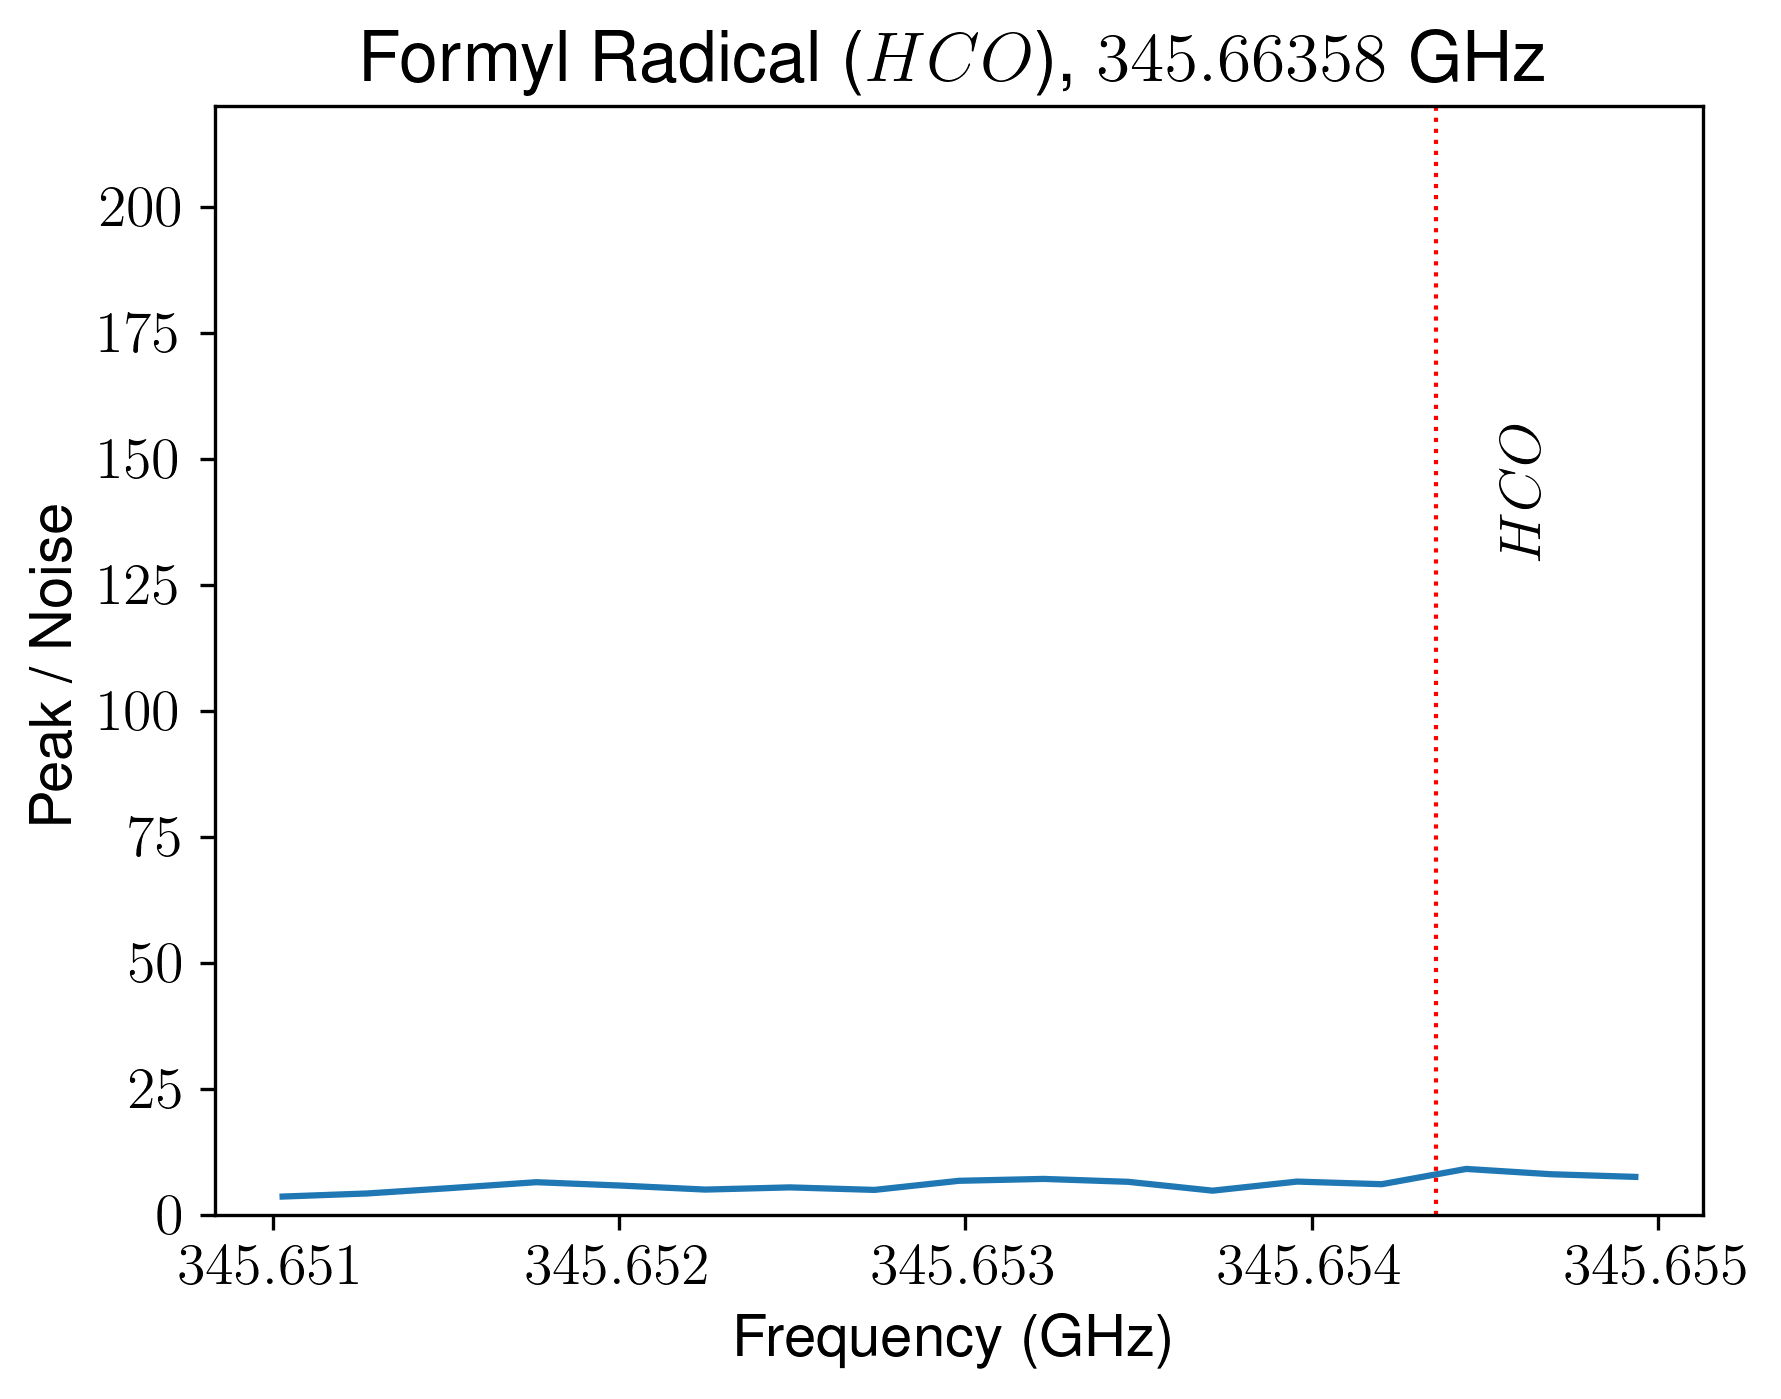
\includegraphics[width=0.245\textwidth]{spw3_HCO}
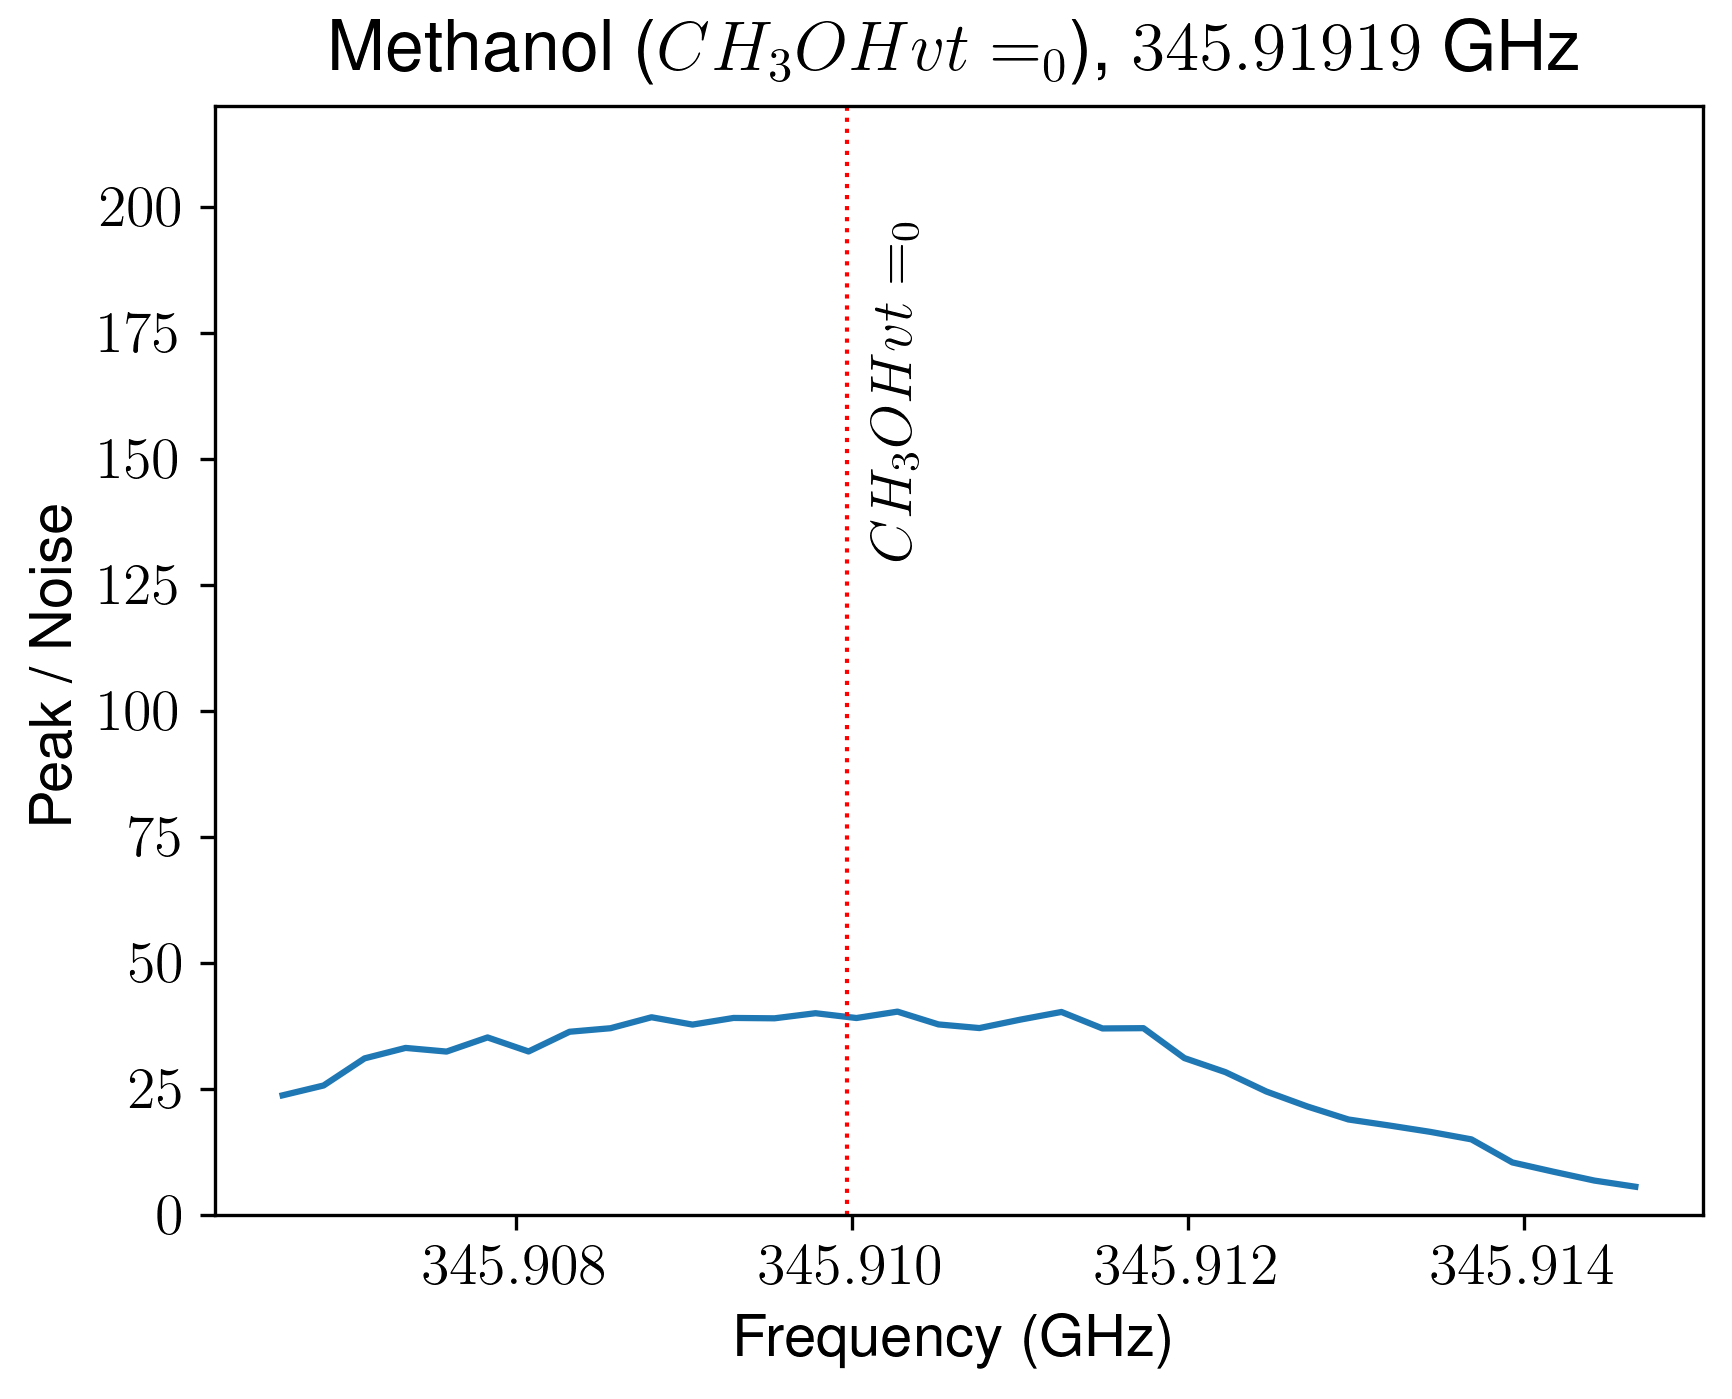
\includegraphics[width=0.245\textwidth]{spw3_CH3OHvt=0}
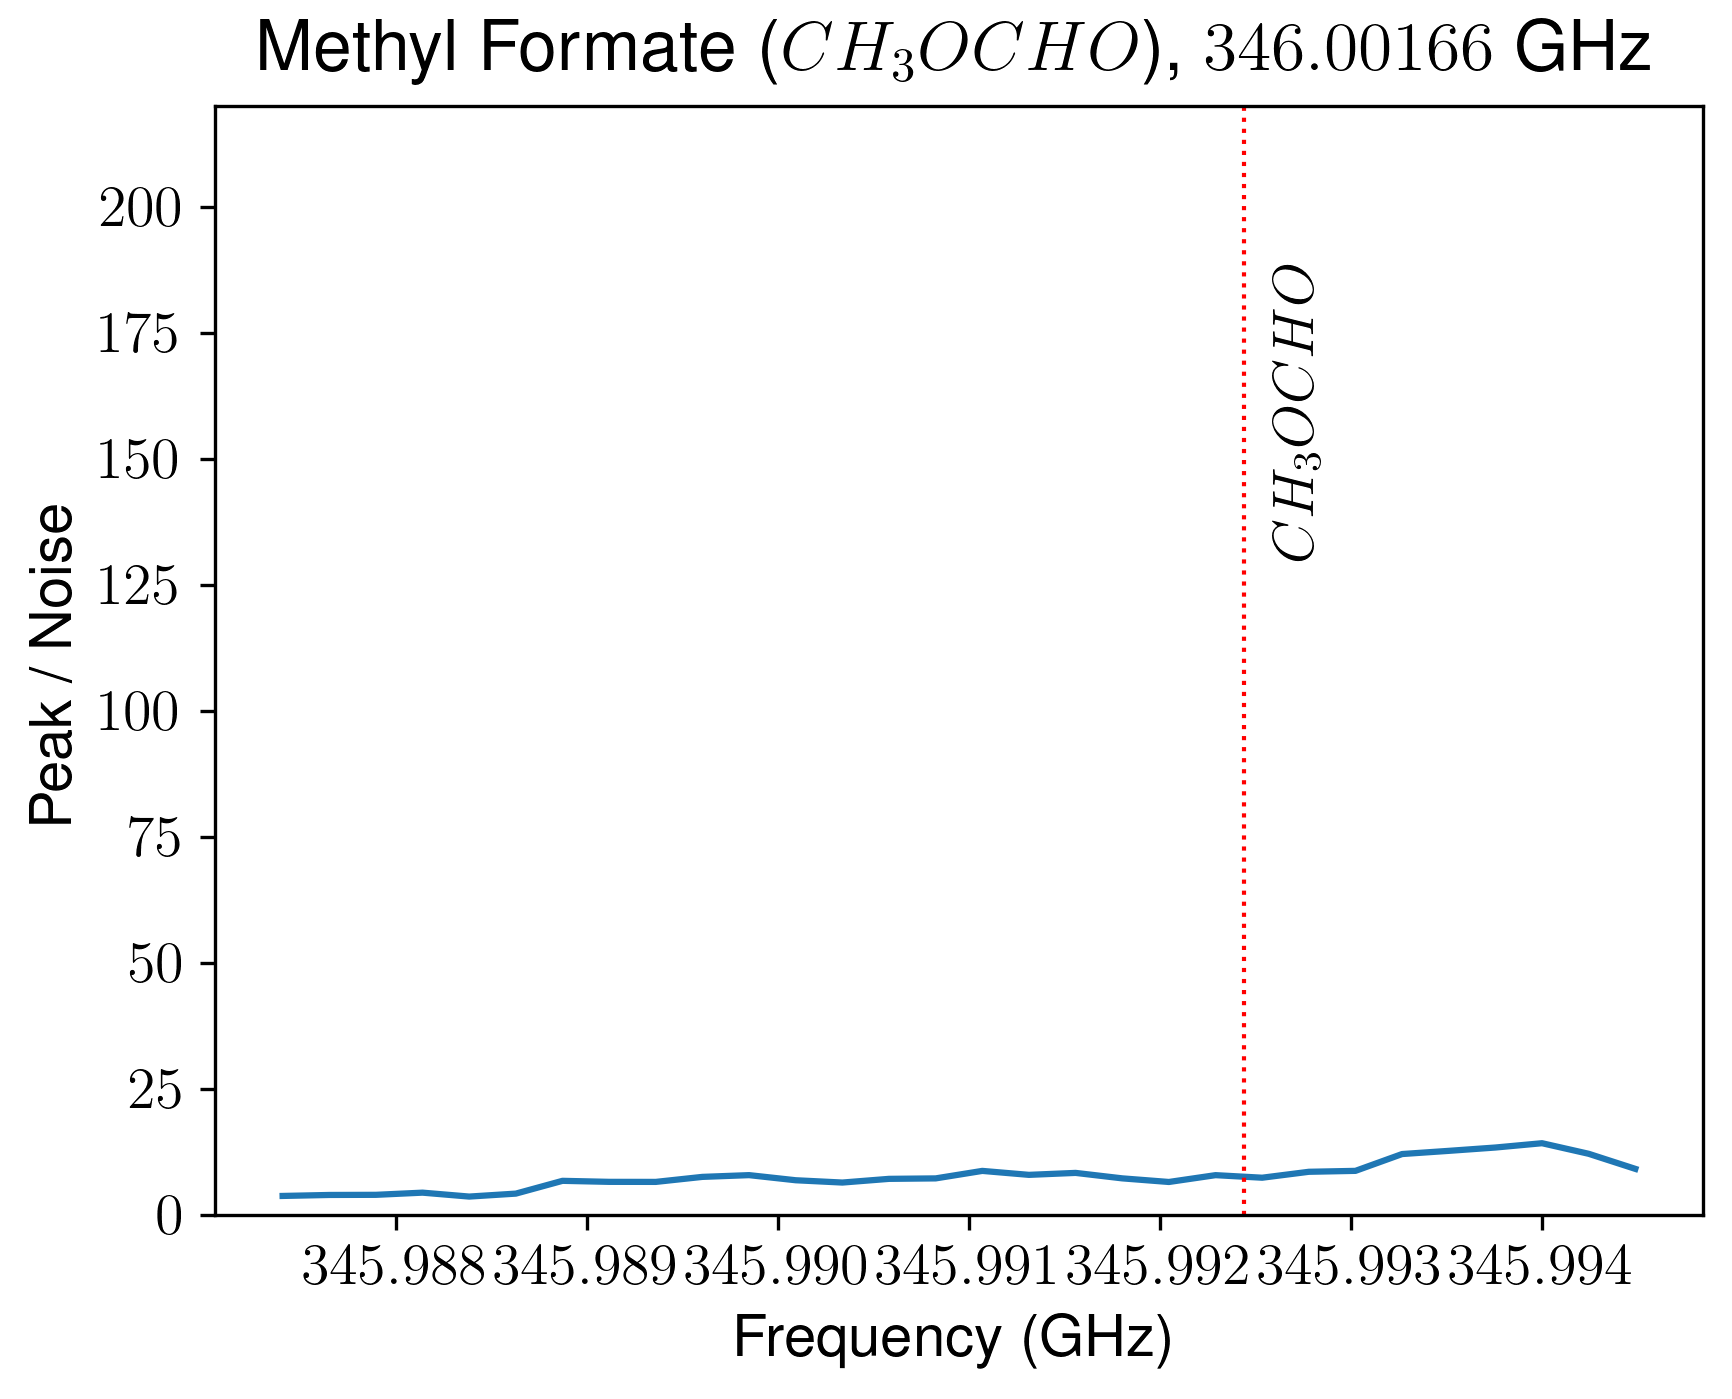
\includegraphics[width=0.245\textwidth]{spw3_CH3OCHO}
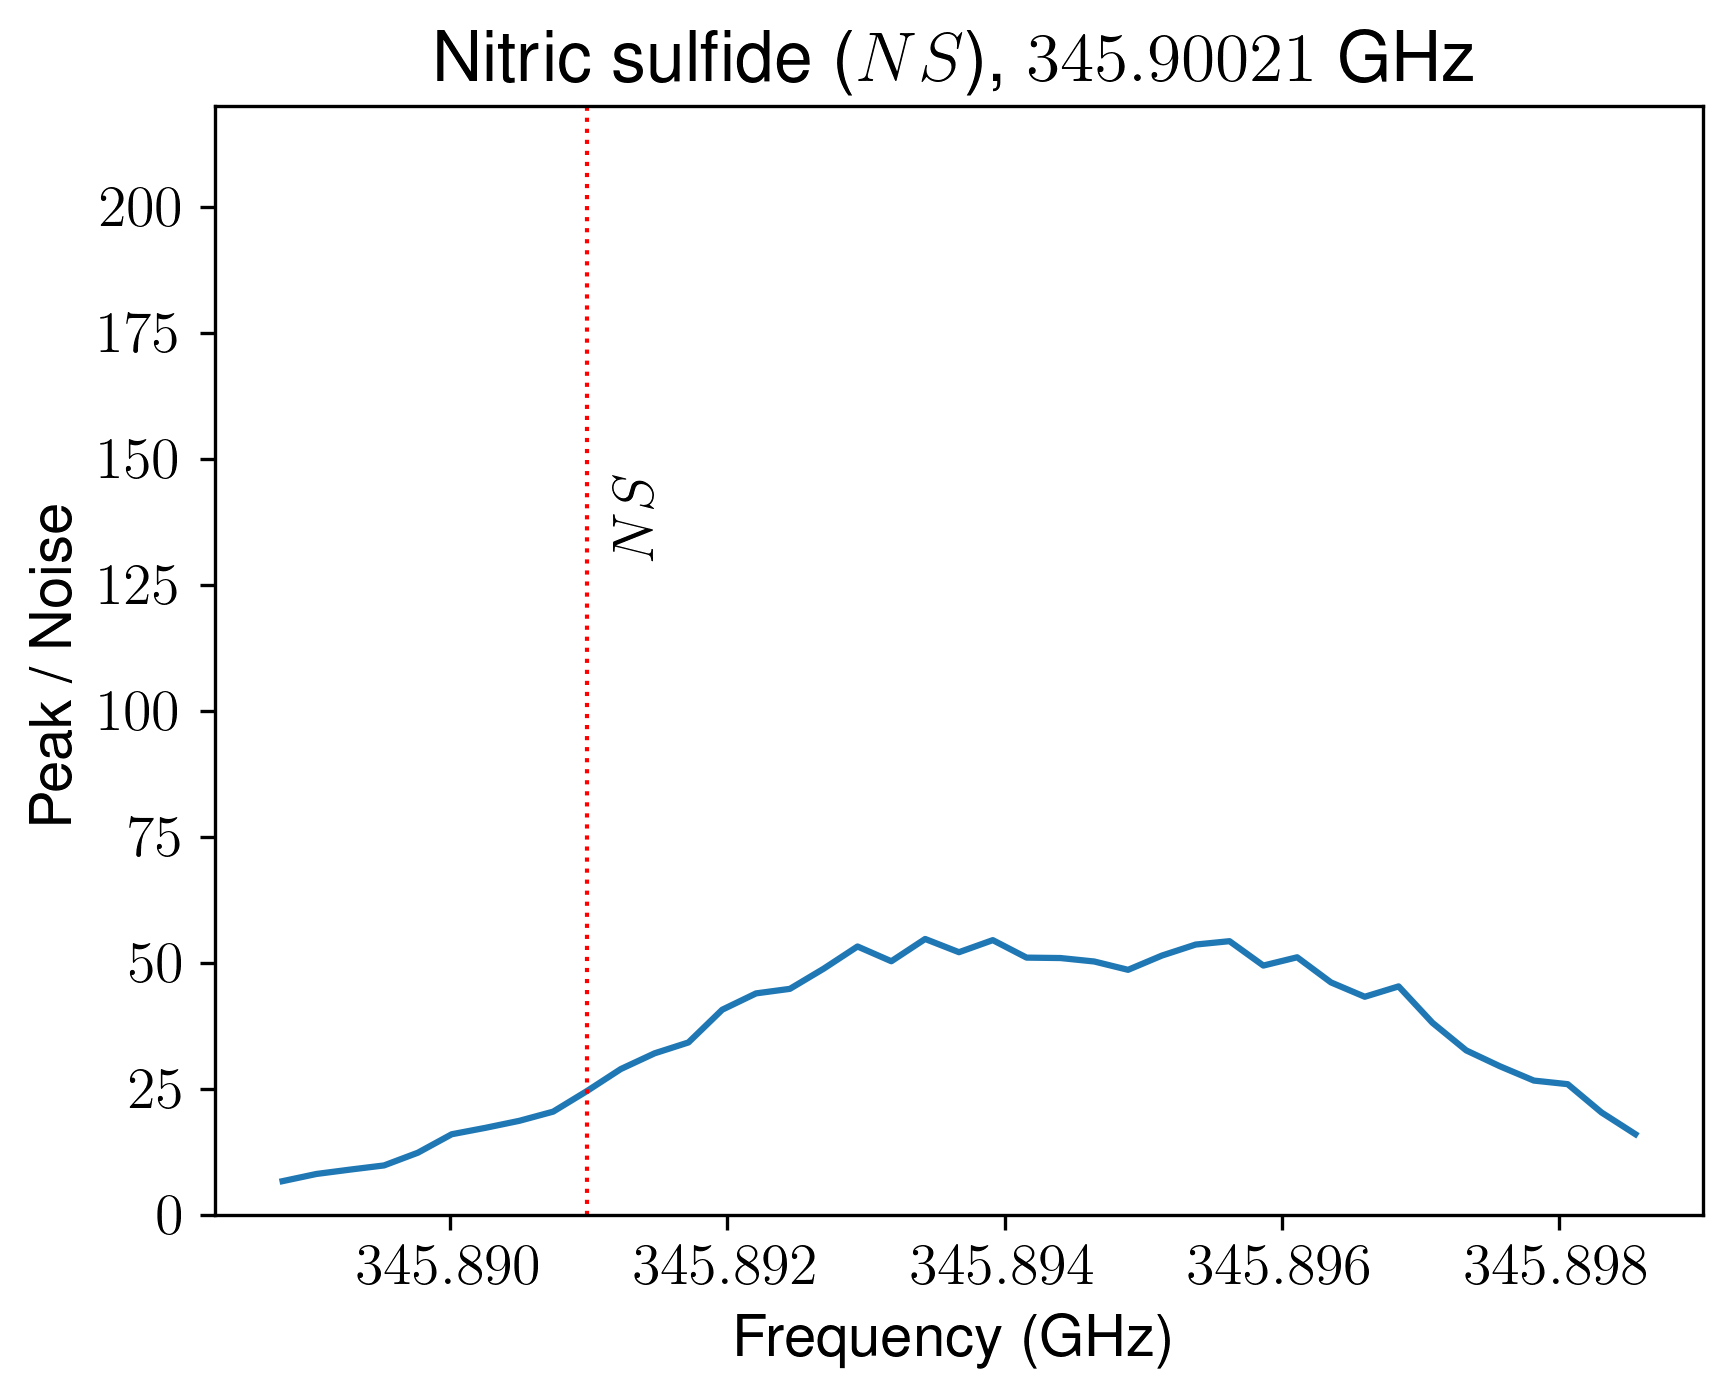
\includegraphics[width=0.245\textwidth]{spw3_NS}
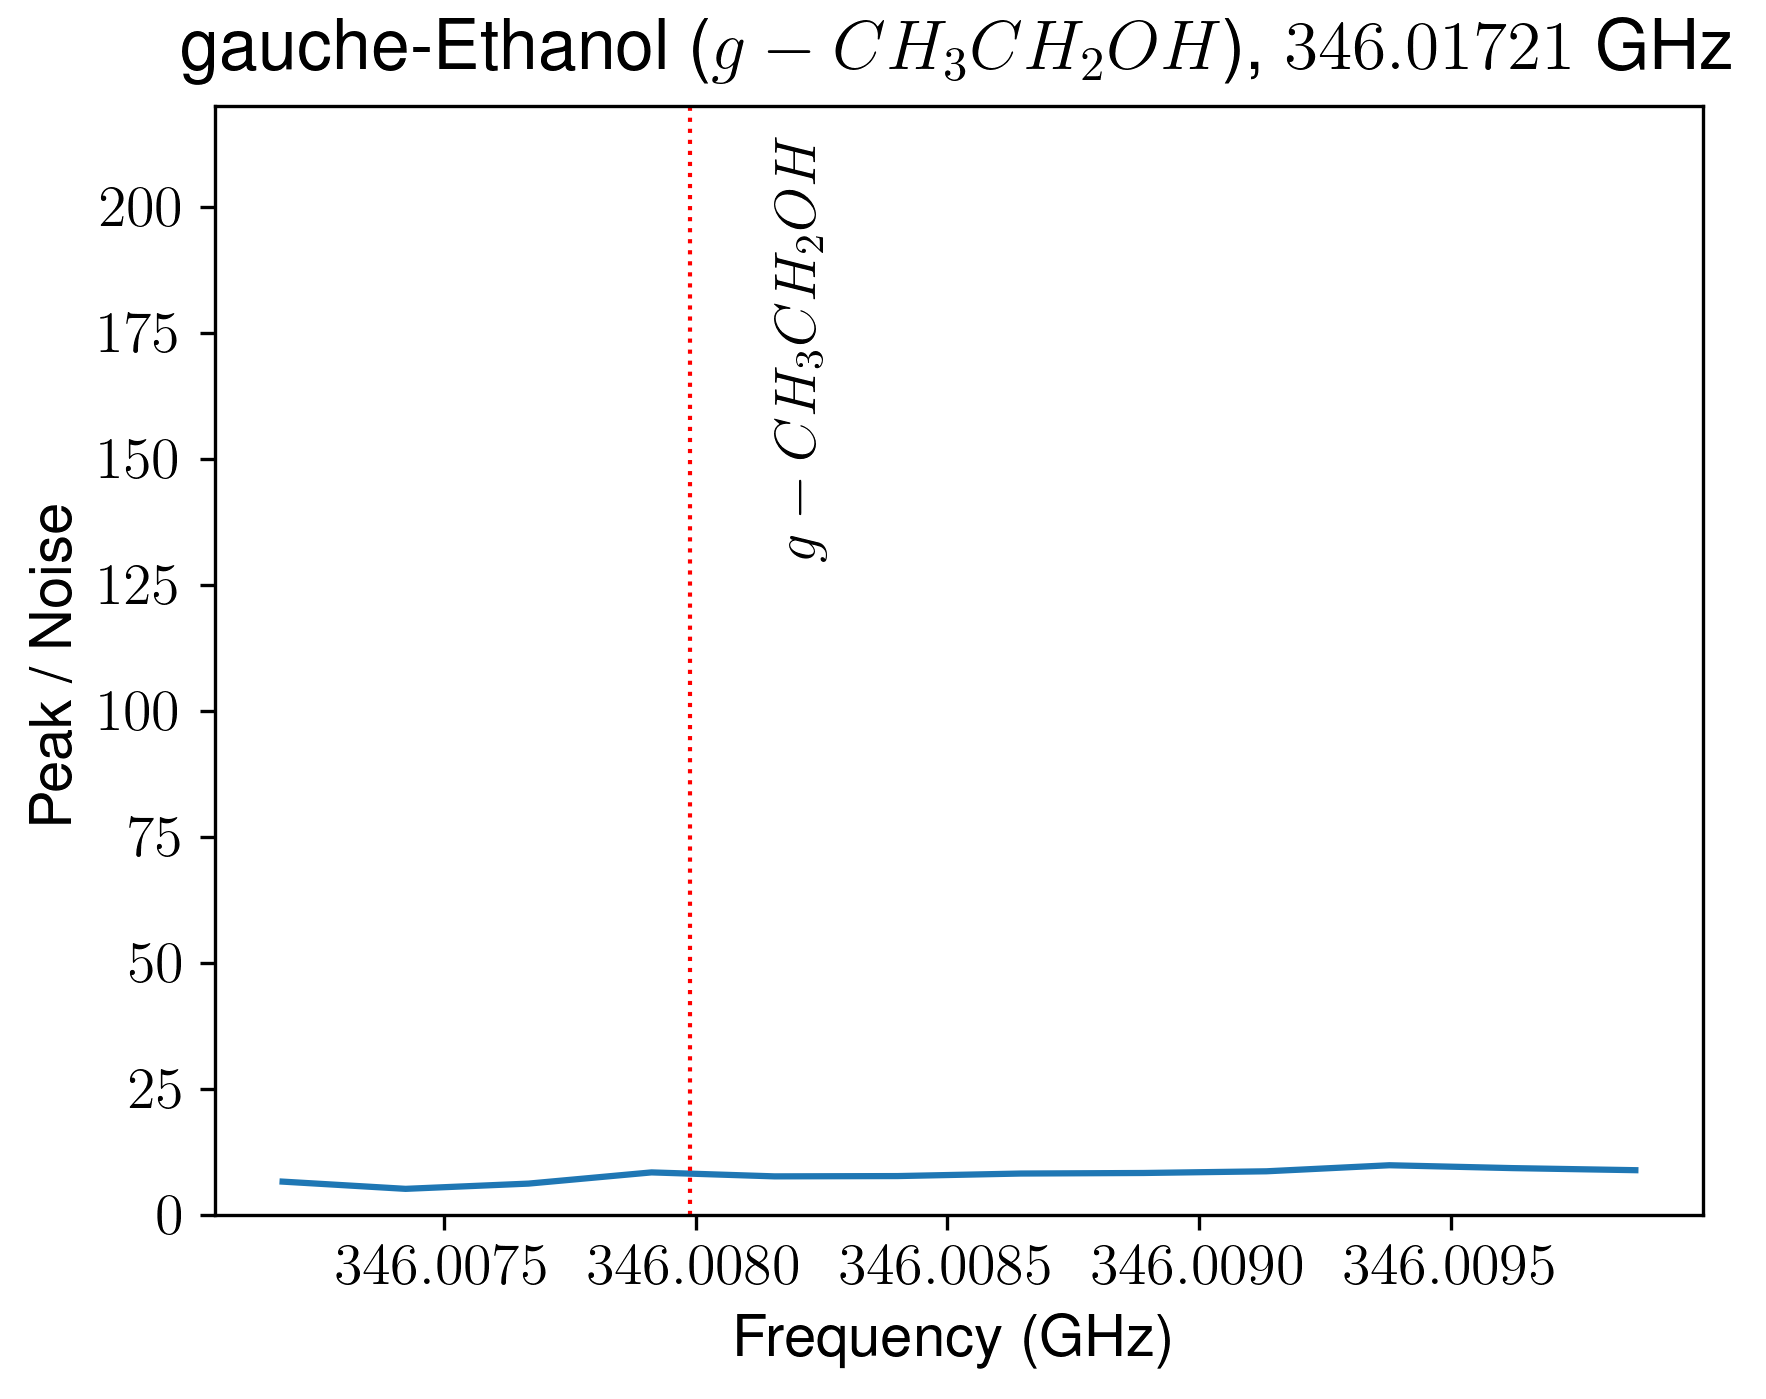
\includegraphics[width=0.245\textwidth]{spw3_g-CH3CH2OH}
\end{figure}


\end{document}
